\chapter{CAPÍTULO, NÍVEL 1}
\label{chap:nivel1}

    Toda seção deve conter um corpo de texto, obrigatoriamente. Insira um novo capítulo com o comando \verb|\chapter{<título>}|, substituindo \verb|<título>| pelo título do capítulo. Use o comando \verb|label{<chave>}| logo após \verb|\chapter{}| para utilizar referência cruzada. O \autoref{qua:intro} mostra um exemplo de código. Observação: se utilizar o sumário tradicional (veja a declaração \verb|\documentclass[]{}| no arquivo \verb|main.tex|) escreva o título capitalizado para garantir que os títulos fiquem em maiúsculo no sumário. Essa observação também é válida para seções e subseções.
    
\begin{quadro}[!htb]
    \centering
    \caption{Exemplo de novo capítulo \label{qua:intro}}
    \begin{tabular}{|c|l|}
        \hline
        1 &\verb|\chapter{Introdução}|\\
        2 &\verb|\label{chap:intro}|\\
        3 &\\
        4 &\verb|<texto>|\\
        \hline
    \end{tabular}
    \fonte{Autoria própria}
\end{quadro}

\nomenclature[S]{$T_S$}{Temperatura}
\nomenclature[S]{$X_i$}{Ponto inicial}

\section{SEÇÃO, NÍVEL 2}
\label{sec:nivel2}

    Essa é uma seção, nível 2, do \autoref{chap:nivel1}. Utilize o comando \verb|\section{<título>}| para criar uma nova seção de nível 2. O \autoref{qua:sec} mostra um exemplo de código.
    
    \begin{quadro}[!htb]
    \centering
    \caption{Exemplo de nova seção de nível 2 \label{qua:sec}}
    \begin{tabular}{|c|l|}
        \hline
        1 &\verb|\section{A vida da marmota}|\\
        2 &\verb|\label{sec:marm}|\\
        3 &\\
        4 &\verb|<texto>|\\
        \hline
    \end{tabular}
    \fonte{Autoria própria}
    \end{quadro}
    
\subsection{SUBSEÇÃO, NÍVEL 3}
\label{subsec:nivel3}

    Essa é uma subseção, nível 3, da \autoref{sec:nivel2}. Caso seja necessário criar uma seção desse tipo em seu texto, utilize o comando \verb|\subsection{<título>}| para criar uma nova seção de nível 3. O \autoref{qua:subsec} mostra um exemplo de código.
    
    \begin{quadro}[!htb]
    \centering
    \caption{Exemplo de nova seção de nível 3 \label{qua:subsec}}
    \begin{tabular}{|c|l|}
        \hline
        1 &\verb|\subsection{Onde vivem}|\\
        2 &\verb|\label{sec:viva}|\\
        3 &\\
        4 &\verb|<texto>|\\
        \hline
    \end{tabular}
    \fonte{Autoria própria}
    \end{quadro}
    
\subsubsection{SUBSEÇÃO, NÍVEL 4}
\label{subsubsec:nivel4}

    Essa é uma subseção, nível 4, da \autoref{subsec:nivel3}. Caso seja necessário criar uma seção desse tipo em seu texto, utilize o comando \verb|\subsubsection{<título>}| para criar uma nova seção de nível 4. O \autoref{qua:subsubsec} mostra um exemplo de código.
    
    \begin{quadro}[!htb]
    \centering
    \caption{Exemplo de nova seção de nível 4 \label{qua:subsubsec}}
    \begin{tabular}{|c|l|}
        \hline
        1 &\verb|\subsubsection{O que comem}|\\
        2 &\verb|\label{sec:food}|\\
        3 &\\
        4 &\verb|<texto>|\\
        \hline
    \end{tabular}
    \fonte{Autoria própria}
    \end{quadro}
    
\subsubsubsection{SUBSEÇÃO, NÍVEL 5}
\label{subsubsubsec:nivel5}

    Isso é uma subseção, nível 5, da \autoref{subsubsec:nivel4}. Pela norma da Associação Brasileira de Normas Técnicas (ABNT), \nomenclature[A]{ABNT}{Associação Brasileira de Normas Técnicas} subseções são permitidas até o nível 5 \cite{NBR6024:2012}. Caso seja necessário criar uma seção desse tipo em seu texto, utilize o comando \verb|\subsubsubsection{<título>}| para criar uma nova seção de nível 5. O \autoref{qua:subsubsubsec} mostra um exemplo de código.
    
    \begin{quadro}[!htb]
    \centering
    \caption{Exemplo de nova seção de nível 5 \label{qua:subsubsubsec}}
    \begin{tabular}{|c|l|}
        \hline
        1 &\verb|\subsubsubsection{Como se reproduzem}|\\
        2 &\verb|\label{sec:sex}|\\
        3 &\\
        4 &\verb|<texto>|\\
        \hline
    \end{tabular}
    \fonte{Autoria própria}
    \end{quadro}
    
\section{SIGLAS, ACRÔNIMOS E SÍMBOLOS}
\label{sec:siglas}

    Para acrescentar uma sigla ou acrônimo na lista de siglas e acrônimos utilize o comando \verb|\nomenclature[A]{<sigla>}{<significado>}| em qualquer parte do texto. É recomendado inserir esse comando logo após a primeira aparição da sigla ou do acrônimo. Um exemplo de código está transcrito no \autoref{qua:siglacode}. 
    
    \begin{quadro}[!htb]
    \centering
    \caption{Exemplo de código para a acrescentar siglas ou acrônimos na lista \label{qua:siglacode}}
    \begin{tabular}{|l|}
        \hline
        \makebox[0.9\linewidth]{\textbf{Código}}\\
        \hline
        \verb|A Ordem dos Advogados do Brasil (OAB) \nomenclature[A]{OAB}{Ordem dos|\\
        \verb|Advogados do Brasil} diz que apoia investigação do ataque de milícias|\\
        \verb|digitais ao Supremo Tribunal Federal (STF) \nomenclature[A]{STF}|\\
        \verb|{Supemo Tribunal Federal}.|\\
        \hline
        \hline
        \makebox[0.9\linewidth]{\textbf{Resultado}}\\
        \hline
        A Ordem dos Advogados do Brasil (OAB) \nomenclature[A]{OAB}{Ordem dos|Advogados do Brasil} diz que apoia investigação do ataque de \\
        milícias digitais ao Supremo Tribunal Federal (STF) \nomenclature[A]{STF}{Supemo Tribunal Federal}.\\
        \hline
    \end{tabular}
    \fonte{Autoria própria}
    \end{quadro}
    
    
    
    
    Para acrescentar um símbolo na lista de símbolos utilize o comando \verb|\nomenclature[S]| \verb|{<simbolo>}{<significado>}| em qualquer parte do texto. É recomendado inserir esse comando logo após a primeira aparição do símbolo. Um exemplo de código está transcrito no \autoref{qua:simbcode}.
    
    \begin{quadro}[!htb]
    \centering
    \caption{Exemplo de código para a acrescentar símbolos na lista \label{qua:simbcode}}
    \begin{tabular}{|l|}
        \hline
        \makebox[0.9\linewidth]{\textbf{Código}}\\
        \hline
        \verb|A segunda lei de Newton diz que $F_r = ma$, onde $F_r$|\\
        \verb|\nomenclature[S]{$F_r$}{Força resultante} é a força resultante, $m$|\\
        \verb|\nomenclature[S]{$m$}{massa} é a massa e $a$ \nomenclature[S]{$a$}|\\
        \verb|{aceleração} é a aceleração.|\\
        \hline
        \hline
        \makebox[0.9\linewidth]{\textbf{Resultado}}\\
        \hline
        A segunda lei de Newton diz que $F_r = ma$, onde $F_r$ \nomenclature[S]{$F_r$}{Força resultante} é a força resultante,\\
        $m$ \nomenclature[S]{$m$}{massa} é a massa e $a$ \nomenclature[S]{$a$}{aceleração} é a aceleração.\\
        \hline
    \end{tabular}
    \fonte{Autoria própria}
    \end{quadro}
    
    Para que as listas sejam geradas é necessário que o comando \textit{\textbf{makeindex}} seja executado com os seguintes argumentos: 
    
    \makebox[0.95\linewidth]{makeindex -s nomencl.ist -o main.nls main.nlo}
    
    \noindent onde ``main'' é o nome do arquivo principal do projeto. Procure mais informações na base de dados do seu editor e copilador \LaTeX.
    
    
\section{SOBRE AS REFERÊNCIAS CRUZADAS E ITENS NUMERADOS}
\label{sec:refs}

    A numeração sequencial de figuras, tabelas, quadros e equações ocorre de modo automático. As ilustrações (figuras), tabelas e quadros serão indexadas automaticamente em suas respectivas listas. 

    Referências cruzadas são obtidas através dos comandos \verb|\label{}| e \verb|\ref{}|. Sendo assim, não é necessário por exemplo, saber que o número de certo capítulo para colocar o seu número no texto. O comando \verb|\autoref{}| facilita referenciação de elementos numerados no texto sem a necessidade de nomear o tipo do elemento.
    
    Observe que este capítulo recebeu a chave ``chap:nivel1'' através do comando \verb|\label{}| (\verb|\label{chap:nivel1}|). Dessa forma, ao utilizar o código \verb|\ref{chap:nivel1}| resulta na escrita do número do capítulo que nesse caso é ``\ref{chap:nivel1}''. De forma análoga, o comando \verb|\autoref{chap:nivel1}| resulta em ``\autoref{chap:nivel1}''.
    
\section{FIGURAS}
\label{sec:figuras}

    Esta seção trata de um exemplo de como inserir uma figura. Note que a \autoref{fig:figura-exemplo1} aparece automaticamente na lista de figuras. Para saber mais sobre o uso de imagens no \LaTeX{} consulte literatura especializada \cite{Goossens2007}.

    \begin{figure}[!htb]
        \centering
        \caption{Exemplo de Figura}
        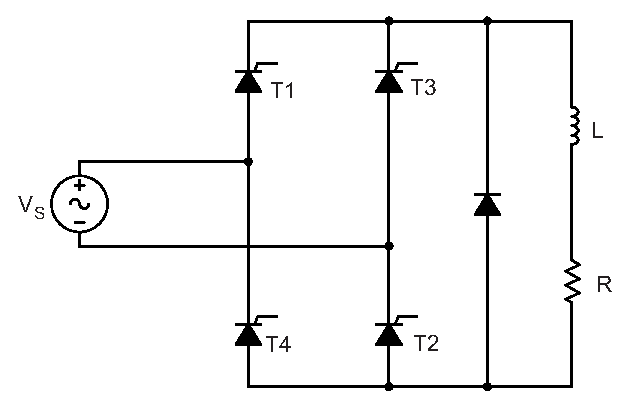
\includegraphics[width=0.6\textwidth]{Caps/Figs/exemplo.eps}
        \fonte{Autoria Própria}
        \label{fig:figura-exemplo1}
    \end{figure}
    
    O código utilizado para inserir a \autoref{fig:figura-exemplo1} está listado no \autoref{qua:figura}.
    
    \begin{quadro}[!htb]
    \centering
    \caption{Código exemplo utilizado para inserir a \autoref{fig:figura-exemplo1} \label{qua:figura}}
    \begin{tabular}{|c|l|}
        \hline
        1 &\verb|\begin{figure}[!htb]|\\
        2 &\verb|\centering|\\
        3 &\verb|\caption{Exemplo de Figura}|\\
        4 &\verb|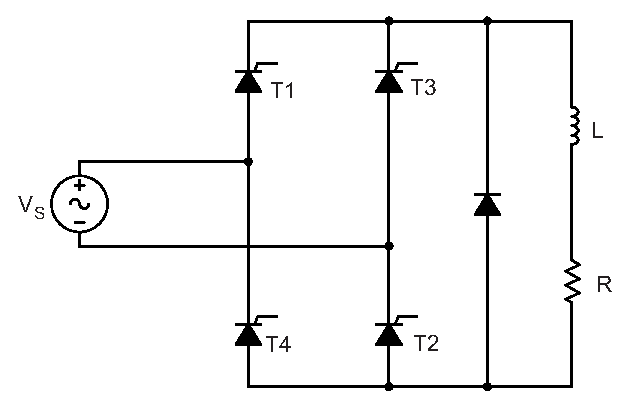
\includegraphics[width=0.6\textwidth]{Caps/Figs/exemplo.eps}|\\
        5 &\verb|\fonte{Autoria Própria}|\\ 
        6 &\verb|\label{fig:figura-exemplo1}|\\ 
        7 &\verb|\end{figure}|\\ 
        \hline
    \end{tabular}
    \fonte{Autoria própria}
    \end{quadro}
    
    Utilize figuras no formato \textit{Encapsulated PostScript} (EPS)\nomenclature[A]{EPS}{\textit{Encapsulated PostScript}}. Caso precise de outro formato, acrescente no preambulo deste modelo o pacote adequado para a sua necessidade.
    
\section{QUADROS E TABELAS}
\label{sec:tabelas}

    Esta seção trata de exemplos de como inserir o \autoref{qua:quadro-exemplo1} e a \autoref{tab:tabela-exemplo1}. Ambos aparecem automaticamente nas suas respectivas listas. Para saber mais informações sobre a construção de tabelas no \LaTeX{} consulte literatura especializada \cite{Mittelbach2004}.

    \begin{quadro}[!htb]
    \centering
    \caption{Exemplo de Quadro \label{qua:quadro-exemplo1}}
    \begin{tabular}{|p{7cm}|p{7cm}|}
        \hline
        \textbf{BD Relacionais} & \textbf{BD Orientados a Objetos} \\
        \hline
        Os dados são passivos, ou seja, certas operações limitadas podem ser automaticamente acionadas quando os dados são usados. Os dados são ativos, ou seja, as solicitações fazem com que os objetos executem seus métodos. & Os processos que usam dados mudam constantemente. \\
        \hline
    \end{tabular}
    \fonte{\citeonline{Barbosa2004}}
    \end{quadro}

    A diferença entre quadro e tabela está no fato que um quadro é formado por linhas horizontais e verticais. Deve ser utilizado quando o conteúdo é majoritariamente não-numérico. O número do quadro e o título vem acima do quadro, e a fonte, deve vir abaixo. Uma tabela é formada apenas por linhas verticais. Deve ser utilizada quando o conteúdo é majoritariamente numérico. O número da tabela e o título vem acima da tabela, e a fonte, deve vir abaixo, tal como no quadro.

    \begin{table}[!htb]
    \centering
    \caption[Resultado dos testes]{Resultado dos testes
    \label{tab:tabela-exemplo1}}
    \begin{tabular}{rrrrr}
        \toprule
            & Valores 1 & Valores 2 & Valores 3 & Valores 4 \\
        \midrule
            Caso 1 & 0,86 & 0,77 & 0,81 & 163 \\
            Caso 2 & 0,19 & 0,74 & 0,25 & 180 \\
            Caso 3 & 1,00 & 1,00 & 1,00 & 170 \\
        \bottomrule
    \end{tabular}
    \fonte{\citeonline{Barbosa2004}}
    \end{table}
    
    Os códigos para inserção do \autoref{qua:quadro-exemplo1} e da \autoref{tab:tabela-exemplo1} estão disponíveis nos Quadros \ref{qua:quaex} e \ref{qua:tabex}.
    
    \begin{quadro}[!htb]
    \centering
    \caption{Código exemplo utilizado para inserir o \autoref{qua:quadro-exemplo1} \label{qua:quaex}}
    \begin{tabular}{|p{0.9\linewidth}|}
    \hline
    \begin{verbatim}
\begin{quadro}[!htb]
\centering
\caption{Exemplo de Quadro \label{qua:quadro-exemplo1}}
    \begin{tabular}{|p{7cm}|p{7cm}|}
    \hline
    \textbf{BD Relacionais} & \textbf{BD Orientados a Objetos} \\
    \hline
    Os dados são passivos, ou seja, certas operações limitadas 
    podem ser automaticamente acionadas quando os dados são 
    usados. Os dados são ativos, ou seja, as solicitações fazem 
    com que os objetos executem seus métodos. & Os processos 
    que usam dados mudam constantemente. \\
    \hline
    \end{tabular}
\fonte{\citeonline{Barbosa2004}}
\end{quadro}
    \end{verbatim}
    \\
    \hline
    \end{tabular}
    \fonte{Autoria própria}
    \end{quadro}
    
    \begin{quadro}[!htb]
    \centering
    \caption{Código exemplo utilizado para inserir a \autoref{tab:tabela-exemplo1} \label{qua:tabex}}
    \begin{tabular}{|p{0.9\linewidth}|}
    \hline
    \begin{verbatim}
\begin{table}[!htb]
\centering
\caption[Resultado dos testes]{Resultado dos testes
\label{tab:tabela-exemplo1}}
    \begin{tabular}{rrrrr}
        \toprule
            & Valores 1 & Valores 2 & Valores 3 & Valores 4 \\
        \midrule
            Caso 1 & 0,86 & 0,77 & 0,81 & 163 \\
            Caso 2 & 0,19 & 0,74 & 0,25 & 180 \\
            Caso 3 & 1,00 & 1,00 & 1,00 & 170 \\
        \bottomrule
    \end{tabular}
\fonte{\citeonline{Barbosa2004}}
\end{table}
    \end{verbatim}
    \\
    \hline
    \end{tabular}
    \fonte{Autoria própria}
    \end{quadro}
    
\section{EQUAÇÕES}
\label{sec:equacoes}

    Esta seção trata de exemplos de como inserir a Eq. (\ref{eq:equacao-exemplo1}) e a Eq. (\ref{eq:equacao-exemplo2}) no corpo do texto \footnote{Deve-se atentar ao fato de a formatação das equações ficar muito boa esteticamente.}. Observe que foram utilizadas duas formas distintas para referenciar as equações. Os códigos utilizados estão no \autoref{qua:eqex}.

    \begin{equation}
        X(s) = \int\limits_{t = -\infty}^{\infty} x(t)  \mathrm{e}^{-st}  dt
        \label{eq:equacao-exemplo1}
    \end{equation}

    \begin{equation}
        F(u, v) = \sum_{m = 0}^{M - 1} \sum_{n = 0}^{N - 1} f(m, n) \exp \left[ -j 2 \pi \left( \frac{u m}{M} + \frac{v n}{N} \right) \right]
        \label{eq:equacao-exemplo2}
    \end{equation}
    
    \begin{quadro}[!htb]
    \centering
    \caption{Código exemplo utilizado para inserir as Equações (\ref{eq:equacao-exemplo1}) e (\ref{eq:equacao-exemplo2}) \label{qua:eqex}}
    \begin{tabular}{|p{0.9\linewidth}|}
    \hline
    \begin{verbatim}
\begin{equation}
    X(s) = \int\limits_{t = -\infty}^{\infty} x(t)\text{e}^{-st}dt
    \label{eq:equacao-exemplo1}
\end{equation}

\begin{equation}
    F(u, v) = \sum_{m = 0}^{M - 1} \sum_{n = 0}^{N - 1} f(m, n) 
    \exp \left[ -j 2 \pi \left( \frac{u m}{M} + \frac{v n}{N} 
    \right) \right]
    \label{eq:equacao-exemplo2}
\end{equation}
    \end{verbatim}
    \\
    \hline
    \end{tabular}
    \fonte{Autoria própria}
    \end{quadro}
    
\section{SOBRE AS LISTAS}
\label{sec:apSobreLista}

    Exemplo de duas listas não numeradas aninhadas, utilizando o comando \verb|\itemize|. Observe a indentação, bem como a mudança automática do tipo de "\textit{bullet}"{} nas listas aninhadas.

    \begin{itemize}
        \item item não numerado 1
        \item item não numerado 2
        \begin{itemize}
            \item subitem não numerado 1
            \item subitem não numerado 2
            \item subitem não numerado 3
        \end{itemize}
        \item item não numerado 3
    \end{itemize}

    Exemplo de duas listas numeradas aninhadas, utilizando o comando \verb|\enumerate|. Observe a numeração progressiva e indentação das listas aninhadas.

    \begin{enumerate}
        \item item numerado 1
        \item item numerado 2
        \begin{enumerate}
            \item subitem numerado 1
            \item subitem numerado 2
            \item subitem numerado 3
        \end{enumerate}
        \item item numerado 3
    \end{enumerate}
    
\subsection{CITAÇÕES INDIRETAS}
\label{subsec:citacoesLivres}

    É a transcrição, com suas próprias palavras, das idéias de um autor, mantendo-se o sentido original. A citação indireta é a maneira que o pesquisador tem de ler, compreender e gerar conhecimento a partir do conhecimento de outros autores. Quanto à chamada da referência, ela pode ser feita de duas maneiras distintas, conforme o nome do(s) autor(es) façam parte do seu texto ou não. Exemplo de chamada fazendo parte do texto:
    
    \vspace{1cm}
    
    Enquanto \citeonline{Maturana2003} defendem uma epistemologia baseada na biologia. Para os autores, é necessário rever \ldots
    
    \vspace{1cm}

    A chamada de referência foi feita com o comando \verb|\citeonline{chave}|, que produzirá a formatação correta.

    A segunda forma de fazer uma chamada de referência deve ser utilizada quando se quer evitar uma interrupção na sequência do texto, o que poderia, eventualmente, prejudicar a leitura. Assim, a citação é feita e imediatamente após a obra referenciada deve ser colocada entre parênteses. Porém, neste caso específico, o nome do autor deve vir em caixa alta, seguido do ano da publicação. Exemplo de chamada não fazendo parte do texto:
    
    \vspace{1cm}
    
    Há defensores da epistemologia baseada na biologia que argumentam em favor da necessidade de \ldots \cite{Maturana2003}.
    
    \vspace{1cm}
    
    Nesse caso a chamada de referência deve ser feita com o comando \verb|\cite{chave}|, que produzirá a formatação correta.
    
\subsection{CITAÇÕES DIRETAS}
\label{subsec:citacoesLiterais}

    É a transcrição ou cópia de um parágrafo, de uma frase, de parte dela ou de uma expressão, usando exatamente as mesmas palavras adotadas pelo autor do trabalho consultado.

    Quanto à chamada da referência, ela pode ser feita de qualquer das duas maneiras já mencionadas nas citações indiretas, conforme o nome do(s) autor(es) façam parte do texto ou não. Há duas maneiras distintas de se fazer uma citação direta, conforme o trecho citado seja longo ou curto.

    Quando o trecho citado é longo (4 ou mais linhas) deve-se usar um parágrafo específico para a citação, na forma de um texto recuado (4 cm da margem esquerda), com tamanho de letra menor e espaçamento entrelinhas simples. Exemplo de citação longa:
    
    \vspace{1cm}
    
    \begin{citacao}
        Desse modo, opera-se uma ruptura decisiva entre a reflexividade filosófica, isto é a possibilidade do sujeito de pensar e de refletir, e a objetividade científica. Encontramo-nos num ponto em que o conhecimento científico está sem consciência. Sem consciência moral, sem consciência reflexiva e também subjetiva. Cada vez mais o desenvolvimento extraordinário do conhecimento científico vai tornar menos praticável a própria possibilidade de reflexão do sujeito sobre a sua pesquisa \cite[p.~28]{Silva2000}.
    \end{citacao}

    Para fazer a citação longa deve-se utilizar os seguintes comandos:
    \begin{verbatim}
\begin{citacao}
<texto da citacao>
\end{citacao}
    \end{verbatim}

    No exemplo, para a chamada da referência o comando \verb|\cite[p.~28]{Silva2000}| foi utilizado, visto que os nomes dos autores não são parte do trecho citado. É necessário também indicar o número da página da obra citada que contém o trecho citado.

    Quando o trecho citado é curto (3 ou menos linhas) ele deve inserido diretamente no texto entre aspas. Exemplos de citação curta:
    
    \vspace{1cm}
    
    A epistemologia parte do princípio de que "assumo que não posso fazer referência a entidades independentes de mim para construir meu explicar" \cite[p.~35]{Maturana2003}.
    
    \vspace{1cm}
    
    A epistemologia baseada na biologia de \citeonline[p.~35]{Maturana2003} parte do princípio de que "assumo que não posso fazer referência a entidades independentes de mim para construir meu explicar".
    
\section{SOBRE AS REFERÊNCIAS BIBLIOGRÁFICAS}
\label{sec:apSobreRefer}

    A bibliografia é feita no padrão \textsc{Bib}\TeX{}. As referências são colocadas em um arquivo separado. Neste template as referências são armazenadas no arquivo 

\begin{center}
``references.bib''.
\end{center}

Existem diversas categorias documentos e materiais componentes da bibliografia. A classe abn\TeX{} define as seguintes categorias (entradas):

\begin{verbatim}
@book
@inbook
@article
@phdthesis
@mastersthesis
@monography
@techreport
@manual
@proceedings
@inproceedings
@journalpart
@booklet
@patent
@unpublished
@misc
\end{verbatim}

Cada categoria (entrada) é formatada pelo pacote \citeonline{abnTeX22014d} de uma forma específica. Algumas entradas foram introduzidas especificamente para atender à norma \citeonline{NBR6023:2002}, são elas: \verb|@monography|, \verb|@journalpart|,\verb|@patent|. As demais entradas são padrão \textsc{Bib}\TeX{}. Para maiores detalhes, refira-se a \citeonline{abnTeX22014d}, \citeonline{abnTeX22014b}, \citeonline{abnTeX22014c}.

% NOTAS DE RODAPÉ--------------------------------------------------------------------------
\section{NOTAS DE RODAPÉ}
\label{sec:notasRodape}

As notas de rodapé pode ser classificadas em duas categorias: notas explicativas\footnote{é o tipo mais comum de notas que destacam, explicam e/ou complementam o que foi dito no corpo do texto, como esta nota de rodapé, por exemplo.} e notas de referências. A notas de referências, como o próprio nome ja indica, são utilizadas para colocar referências e/ou chamadas de referências sob certas condições.

\chapter{CRONOGRAMA}
\label{chap:cronograma}

Esse capítulo trata de um exemplo de cronograma:

O desenvolvimento deste trabalho se dará da seguinte forma:

% Atividades
\begin{enumerate}
    % 1
	\item \label{item1} \textbf{Elaboração da proposta de TCC}: Definição do escopo do projeto e determinação da metodologia.
	
	% 2
	\item \label{item2} \textbf{Escrita do texto TCC 1}: Pesquisa sobre grade de Bragg e descrição de todo  processo realizado para a análise dos resultados.
	
	% 3
	\item \label{item3} \textbf{Agendamento e apresentação do TCC 1}: Agendamento e apresentação do trabalho com o professor orientador perante à Banca.
	
	% 4 
	\item \label{item4} \textbf{Revisão do texto}: Correção do trabalho escrito e finalização para entrega à Banca.
	
	% 5
	\item \label{item5} \textbf{Apresentação do TCC 1}: Apresentação do trabalho proposto.
	
	% 6
	\item \label{item6} \textbf{Alterações e entrega do TCC 1}: Entrega do TCC 1 com as devidas alterações solicitadas pela Banca.
	
	% 7
	\item \label{item7} \textbf{Implementação do \textit{firmware} da PCA}: Produção dos códigos do sistema de interrogação para início de análise da velocidade de variação dos transdutores da placa.
	
	% 8
	\item \label{item8} \textbf{Finalizar o projeto da PAL}: Terminar de montar a placa destinada ao acionamento e proteção do laser.
	
	% 9
	\item \label{item9} \textbf{Implementação do \textit{firmware} da PAL}: Desenvolver o controle digital em C que será responsável pela placa e testar seus módulos.
	
	% 10
	\item \label{item10} \textbf{Testes preliminares de comunicação entre placas}: Montagem de ambos os módulos desenvolvidos neste trabalho, a PCA e a PAL, para iniciar ensaios e verificar a maneira como os sinais são transmitidos pelo circuito.
	
	% 11
	\item \label{item11} \textbf{Experimento com a PCA e o ECO}: Montagem da placa de interrogação com o emulador, para iniciar teste do controle digital e decidir quais serão os parâmetros destinados aos transdutores. 
	
	% 12
	\item \label{item12} \textbf{Planejar protocolo de comunicação}: Desenvolver a tabela de instruções que será destinada a intercomunicação da PCA e do ECO com o computador.
	
	% 13
	\item \label{item13} \textbf{Teste do sistema completo}: Instalação de todos os módulos e início dos testes com as três placas para certificar a metodologia descrita ao longo do trabalho.
	
	% 14
	\item \label{item14} \textbf{Análises das técnicas de pós-processamento}: Elaboração do procedimento que será implementado no computador para o pós-processamento dos sinais questionados e transmitidos via comunicação RS-485.
	
	% 15
    \item \label{item15} \textbf{Desenvolvimento da interface gráfica}: Implementar e testar a interface que será utilizada na demonstração dos valores interpretados e do padrão refletido.
    
    % 16
     \item \label{item16} \textbf{Obtenção dos resultados}: Serão obtidos os resultados do funcionamento do sistema para que seja feita a análise e qualquer modificação necessária.
     
     % 17
	\item \label{item17} \textbf{Escrita do texto TCC2}: Escrita dos resultados obtidos nos testes e conclusão do trabalho. 
	
	% 18
	\item \label{item18} \textbf{Revisão do texto e entrega}: Realização das devidas modificações solicitadas pela Banca e entrega do trabalho.
	
	% 19
	\item \label{item19} \textbf{Apresentação do TCC2}: Apresentação do trabalho.
	
	% 20
    \item \label{item20} \textbf{Alterações e entrega do TCC2}: Entrega do TCC2 com as devidas alterações solicitadas pela Banca.
    

\end{enumerate}

O \autoref{qua:cronograma} mostra o período previsto para as atividades propostas.

\begin{landscape}
\begin{quadro}
\caption{\label{qua:cronograma}Cronograma de atividades}
\begin{tabular}{ccccccccccccl}
   Atividade & Ago/18               & Set/18               & Out/18               & Nov/18               & Dez/18               & Jan/19               & Fev/19               & Mar/19               & Abr/19               & Maio/19              & Jun/19               &  \\
   & \multicolumn{1}{l}{} & \multicolumn{1}{l}{} & \multicolumn{1}{l}{} & \multicolumn{1}{l}{} & \multicolumn{1}{l}{} & \multicolumn{1}{l}{} & \multicolumn{1}{l}{} & \multicolumn{1}{l}{} & \multicolumn{1}{l}{} & \multicolumn{1}{l}{} & \multicolumn{1}{l}{} &  \\ \cline{1-12}
   & \multicolumn{1}{l}{} & \multicolumn{1}{l}{} & \multicolumn{1}{l}{} & \multicolumn{1}{l}{} & \multicolumn{1}{l}{} & \multicolumn{1}{l}{} & \multicolumn{1}{l}{} & \multicolumn{1}{l}{} & \multicolumn{1}{l}{} & \multicolumn{1}{l}{} & \multicolumn{1}{l}{} &  \\
\ref{item1}  & X                    &                      &                      &                      &                      &                      &                      &                      &                      &                      &                      &  \\
\ref{item2}  &                      & X                    &                      &                      &                      &                      &                      &                      &                      &                      &                      &  \\
\ref{item3}  &                      & X                    & X                 &                      &                      &                      &                      &                      &                      &                      &                      &  \\
\ref{item4}  &                      & X                    & X                    &                      &                      &                      &                      &                      &                      &                      &                      &  \\
\ref{item5}  &                      &                      & X                    &                      &                      &                      &                      &                      &                      &                      &                      &  \\
\ref{item6}  &                      &                      & X                    &                      &                      &                      &                      &                      &                      &                      &                      &  \\
\ref{item7}  &                      &                      & X                    & X                    &                      &                      &                      &                      &                      &                      &                      &  \\
\ref{item8}  &                      &                      & X                    & X                    &                      &                      &                      &                      &                      &                      &                      &  \\
\ref{item9}  &                      &                      & X                    & X                    &                      &                      &                      &                      &                      &                      &                      &  \\
\ref{item10} &                      &                      &                      & X                    & X                    &                      &                      &                      &                      &                      &                      &  \\
\ref{item11} &                      &                      &                      &                      & X                    & X                    &                      &                      &                      &                      &                      &  \\
\ref{item12} &                      &                      &                      &                      & X                    &                      &                      &                      &                      &                      &                      &  \\
\ref{item13} &                      &                      &                      &                      &                      & X                    & X                    & X                    & X                    &                      &                      &  \\
\ref{item14} &                      &                      &                      &                      &                      &                      & X                    & X                    & X                    &                      &                      &  \\
\ref{item15} &                      &                      &                      &                      &                      &                      & X                    & X                    & X                    &                      &                      &  \\
\ref{item16} &                      &                      &                      &                      &                      &                      &                      & X                    & X                    &                      &                      &  \\
\ref{item17} &                      &                      &                      &                      &                      &                      &                      &                      & X                    & X                    & X                    &  \\
\ref{item18} &                      &                      &                      &                      &                      &                      &                      &                      & X                    & X                    & X                    &  \\
\ref{item19} &                      &                      &                      &                      &                      &                      &                      &                      &                      & X                    & X                    &  \\
\ref{item20} & \multicolumn{1}{l}{} & \multicolumn{1}{l}{} & \multicolumn{1}{l}{} & \multicolumn{1}{l}{} & \multicolumn{1}{l}{} & \multicolumn{1}{l}{} & \multicolumn{1}{l}{} & \multicolumn{1}{l}{} &                      &                      & X                    &  \\
   & \multicolumn{1}{l}{} & \multicolumn{1}{l}{} & \multicolumn{1}{l}{} & \multicolumn{1}{l}{} & \multicolumn{1}{l}{} & \multicolumn{1}{l}{} & \multicolumn{1}{l}{} & \multicolumn{1}{l}{} & \multicolumn{1}{l}{} & \multicolumn{1}{l}{} & \multicolumn{1}{l}{} &  \\ \cline{1-12}
\end{tabular}
\end{quadro}

\end{landscape}

\clearpage

Outra forma de fazer o cronograma é através do pacote ``pgfgantt''. Informações podem ser encontradas na \href{https://ctan.org/pkg/pgfgantt}{página do projeto}\footnote{https://ctan.org/pkg/pgfgantt}.

